\section{Zielsetzung}
In diesem Versuch soll die Funktionsweise eines HeNe-Lasers untersucht werden. Außerdem werden einige
charakteristische Eigenschaften wie z.B. die Stabilitätsbedingung, die Polarisation und die
Wellenlänge des Lasers bestimmt.

\section{Theorie}
\label{sec:Theorie}
\subsection{Die Funktionsweise}
Jeder Laser besteht aus drei Komponenten, dem aktiven Lasermedium, der Pumpquelle und dem
Resonator. Dieser prinzipielle Aufbau ist in Abbildung \ref{fig:aufbau} zu sehen.
Mit diesen Komponenten ist es möglich monochromatisches Licht hoher Intensität
und Kohärenz zu emittieren.

\begin{figure}[H]
  \centering
  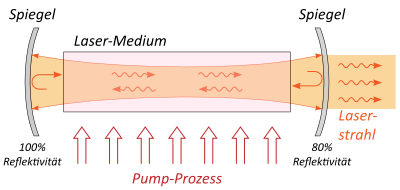
\includegraphics[width=9cm]{Aufbau3.png}
  \caption{Prinzipieller Aufbau eines Lasers \cite{Laser}.}
  \label{fig:aufbau}
\end{figure}

Über das Lasermedium wird das Strahlungsspektrum bestimmt, dies kann vom UV-Bereich bis hin
zum IR-Bereich reichen. Die Pumpquelle wird benötigt, um eine Besetzungsinversion und damit
induzierte Emission zu erzeugen. Der Resonator dient zur optischen Rückkopplung, wodurch das
Licht erneut durch das Lasermedium geschickt wird.

In einem Atom mit zwei Energieniveaus, dem Grundzustand und einem angeregten Zustand, gibt es
drei verschiedene Wechselwirkungen von Photonen, diese sind in Abbildung \ref{fig:Emission} dargestellt.
Ein Photon kann absorbiert werden, wenn es die
Energie des Übergangs hat. Wechselt ein Photon spontan vom angeregten Zustand in den Grundzustand
handelt es sich um spontane Emission. Dieser Vorgang kann auch durch ein einfallendes Photon
stimuliert werden, dann spricht man von stimulierter Emission. Das ausgelöste und das stimulierte Photon
haben dabei die gleiche Energie, Phase und Ausbreitungsrichtung.

\begin{figure}[H]
  \centering
  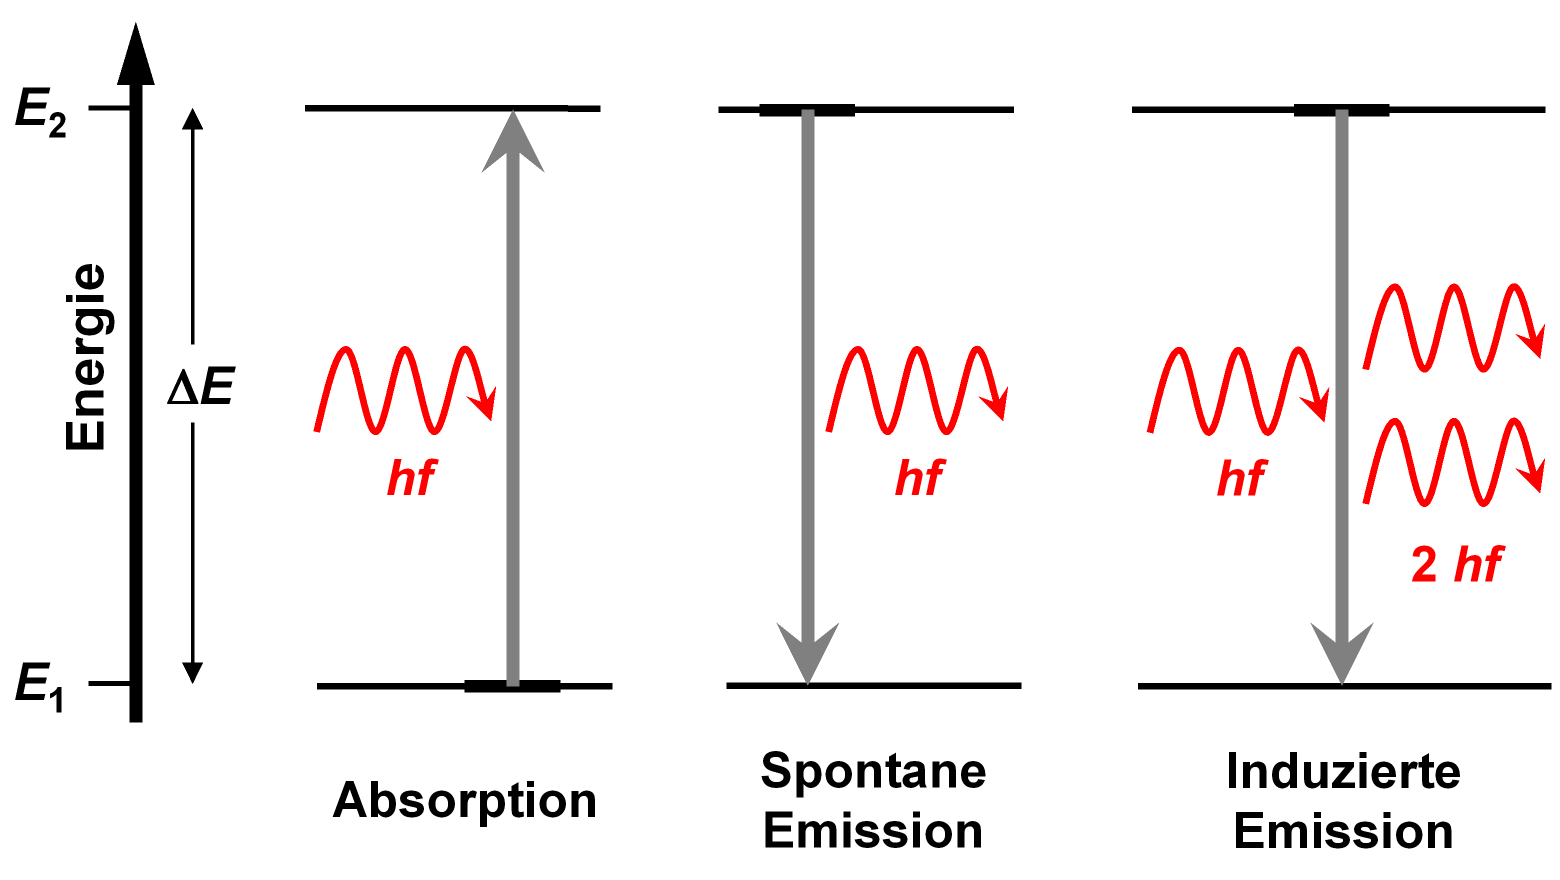
\includegraphics[width=9cm]{Emission.png}
  \caption{Die möglichen Wechselwirkungen von Photonen \cite{seos}.}
  \label{fig:Emission}
\end{figure}

Bei einem Laser wird das Lasermaterial so manipuliert, dass die Wechselwirkung des Strahlungsfeldes
mit dem Lasermaterial zu einer Verstärkung des einfallenden Lichts führt. Dazu muss die stimulierte
Emission der spontanen überwiegen, denn nur dann ist eine hohe Kohärenz und Verstärkung der Strahlung möglich.
Die Voraussetzung für stimulierte Emission ist eine Besetzungsinversion, diese liegt vor, wenn der angeregte Zustand
eine höhere Besetzungszahl aufweist, als der Grundzustand. Aufgrund der Boltzmann-Verteilung ist der Grundzustand im
thermischen Gleichgewicht jedoch stärker besetzt. Um trotzdem eine Besetzungsinversion zu erreichen, wird dem
Lasermedium über die Pumpquelle permanent Energie von außen zugeführt, dies kann über über Elektronenstoß
oder optische Anregung erfolgen.
Da die Verstärkung exponentiell mit dem Laufweg im Lasermedium ansteigt wird ein optischer Resonator verdendet, um den
Laufweg zu maximieren. Der Resonator besteht aus zwei Spiegeln, in dessen Mitte das Laserrohr steht, der Laserstrahl wird an
dem Spiegel reflektiert und durchläuft das Lasermedium somit mehrfach. Einer der Spiegel ist teildurchlässig, um den Laserstrahl
auszukoppeln. Für den Aufbau des Resonators gibt es verschiedene Möglichkeiten, er kann aus planparallelen Spiegeln, spährischen
Spiegeln oder einer Mischung daraus bestehen. Je nach verwendeter Spiegelart spricht man von einem planparallelem oder spährischen
Resonator. Ziel ist es, so einen selbsterregten Oszillator zu erzeugen. Dafür müssen die Verluste durch den Resonator möglichst gering
gehalten werden, dies ist bei einem konfokalen Resonator der Fall, bei dem die Spiegelbrennpunkte zusammenfallen.

Ein stabiler Resonator liegt vor, wenn die Verluste geringer sind als als die Verstärkung durch induzierte Emission.
Dies ist erfüllt, wenn die Stabilitätsbedingung
\begin{equation}
<<<<<<< HEAD
  0< g_1 \cdot g_2 <1
||||||| merged common ancestors
  0< g_1 \cdot g_2 <1.
=======
  0< g_1 \cdot g_2 <1.
  \label{eqn:stab1}
>>>>>>> Fluschedidusch
\end{equation}
erfüllt ist.
Dabei ist der Resonatorparameter
\begin{equation}
  g_i = 1- \frac{L}{r_i}
    \label{eqn:stab2}
\end{equation}
von der Länge des Resonators $L$ und der Krümmung der Resonatorspiegel $r_i$ abhängig.

\subsection{Der HeNe-Laser}
Das Laserrohr des Helium-Neon-Lasers ist mit einem Helium-Neon Gasgemisch im Verhältnis 5:1 gefüllt,
Helium wird als Pumpquelle verwendet und Neon als Lasermedium. An den Enden des Laserrohrs befinden sich
Brewsterfenster, die einen verlustfreien Durchtritt von Licht ermöglichen, indem p-Polarisiertes Lich
durchgelassen und s-Polarisiertes Licht reflektiert wird. Außerdem ist das Laserrohr ist mit Elektroden versehen,
zwischen denen eine Gasentladung stattfindet. Diese Gasentladung bringt die Heliumatome durch Elektronenstoß in einen
langlebigen, metastabilen angeregten Zustand, über Stöße 2. Art wird die Energie der angeregten Heliumatome an die
Neonatome abgegeben:
\begin{equation}
  He^* + Ne \rightarrow He + Ne^* + \Delta E.
\end{equation}
Dabei sind $He^*$ und $Ne^*$ angeregte Zustände. Dieser Vorgang, welcher in Abbildung \ref{fig:entladung} zu sehen ist,
wird auch als Pumpvorgang bezeichnet.

\begin{figure}[H]
  \centering
  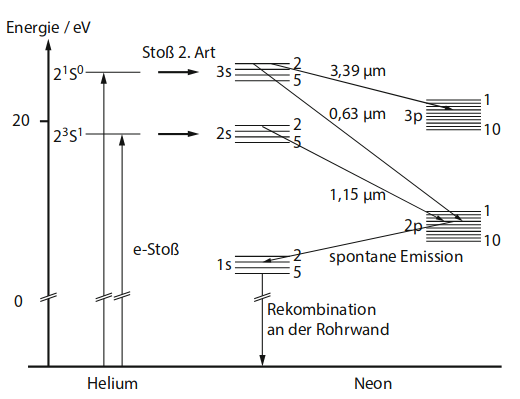
\includegraphics[height=7cm]{Entladung.png}
  \caption{Niveauschema des HeNe-Lasers \cite{springer2}.}
  \label{fig:entladung}
\end{figure}

Die vom HeNe-Laser bekannte rote Laserlinie bei 633\;nm wird durch den Neonübergang $3s_2 \rightarrow 2p_4$
erzeugt.

\subsection{Moden}
Die Resonatorlänge ist viel größer als die Wellenlänge $\lambda$ des Lichts, wodurch viele Frequenzen die
Resonanzbedingung einer stehenden Welle erzeugen.
Die longitudinale Mode des Resonators bezeichnet die Anzahl $q$ der Wellenlängen im Resonator. Es können
auch transversale Moden entstehen, diese werden durch Unebenheiten oder Verkippungen der Spiegel verursacht.
Die Moden werden mit $\text{TEM}_{lpq}$ (TEM=transverse rlectromagnetic mode) bezeichnet. Mit der
transversalen Modenzahl $l$ und $p$ werden dabei die Knoten in x- und y-Richtung bezeichnet,
während die longitudinale Modenzahl $q$ meistens weggelassen wird.
Höhere Moden haben in der Regel größere Verluste als niedrige, deshalb ist die Mode mit den geringsten
Verlusten und der höchsten Symmetrie die Grundmode $\text{TEM}_{00}$.
%Für einen konfokalen Resonator mit runden Spiegeln ist die Feldverteilung gegeben durch:
%\begin{equation}
%  E_{lpq} \sim \cos(l\phi)\frac{(2\rho)^2}{(1+Z^2)^{(1+l)/2}}
%                     L_p^q\left(\frac{(2\rho)^2}{1+Z^2}\right) \exp\left(-\frac{\rho^2}{1+Z^2}\right)\\
%                   \cdot\exp\left(
%                     -i\left(\frac{(1+Z)\pi R}{\lambda}+\frac{\rho^2Z}{1+Z^2}-(l+2p+1)
%                     \left(\frac{\pi}{2}-\arctan\frac{1-Z}{1+Z}\right)\right)\right)
%\end{equation}
%mit
%\begin{align}
%  \rho &= \sqrt{\frac{2\pi}{R\lambda}} \\
%  Z &= \frac{2z}{R}.
%\end{align}
%Dabei bezeichnet $L_p^q(u)$ das Laguerre-Polynom.

Die Intensitätsverteilungen für verschieden Moden sind in Abbildung \ref{fig:TEM} dargestellt.
\begin{figure}[H]
  \centering
  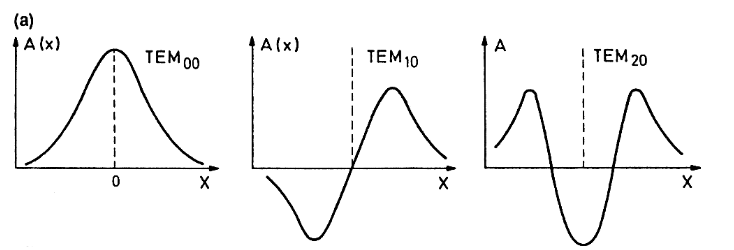
\includegraphics[width=11cm]{TEM.png}
  \caption{Intensitätsverteilung verschiedener Moden \cite{springer}.}
  \label{fig:TEM}
\end{figure}

Die Intensitätsverteilung der $\text{TEM}_{00}$-Grundmode wird durch eine Gaußverteilung der Form
\begin{equation}
  I(r)=I_0\exp{\frac{-2r^2}{\omega^2}}
\end{equation}
beschrieben. Die Maximalintensität wird dabei mit $I_0$ beschrieben und $r$ bezeichnet den Abstand
zur optischen Achse. Mit $2\omega$ wird der Strahldurchmesser beschrieben, dabei lässt dich Strahlradius
wie folgt berechnen:
\begin{equation}
  \omega(z)=\omega_0\sqrt{1+\Big(\frac{\theta_z}{\omega_0}\Big)^2}.
  \label{eqn:Strahlradius}
\end{equation}
Dabei wird mit $\omega_0$ die Strahlweite bezeichnet und mit $z$ der Abstand zu dieser.
Die Stahldivergenz des Gaußschen Strahlers kann über $\theta=(\sfrac{\lambda}{\pi})\cdot\omega_0$ berechnet werden.
